\subsection{User Interface}
The following mockups represent a basic idea of how the users' mobile app will look like in the first 
release. 

\begin{figure}[h!]
	\centering
 	 \begin{minipage}[b]{0.25\textwidth}
    		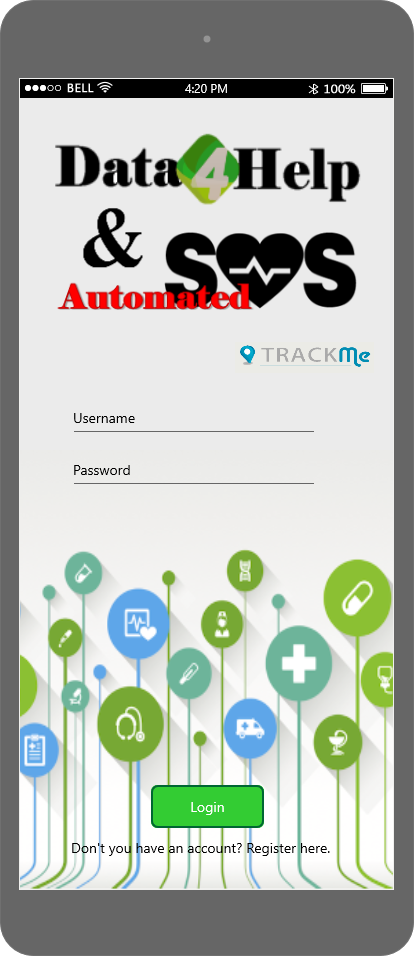
\includegraphics[width=\textwidth]{./pictures/login_user.png}
    		\caption{Mock up - Login screen.}
  	\end{minipage}
	\hfill
 	\begin{minipage}[b]{0.25\textwidth}
    		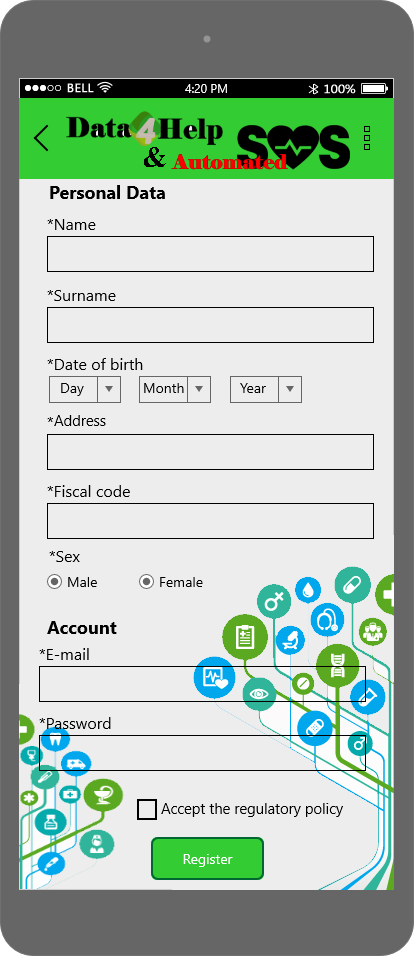
\includegraphics[width=\textwidth]{./pictures/user_registration.png}
    		\caption{Mock up - Registration.}
	\end{minipage}
	\hfill
	\begin{minipage}[b]{0.25\textwidth}
    		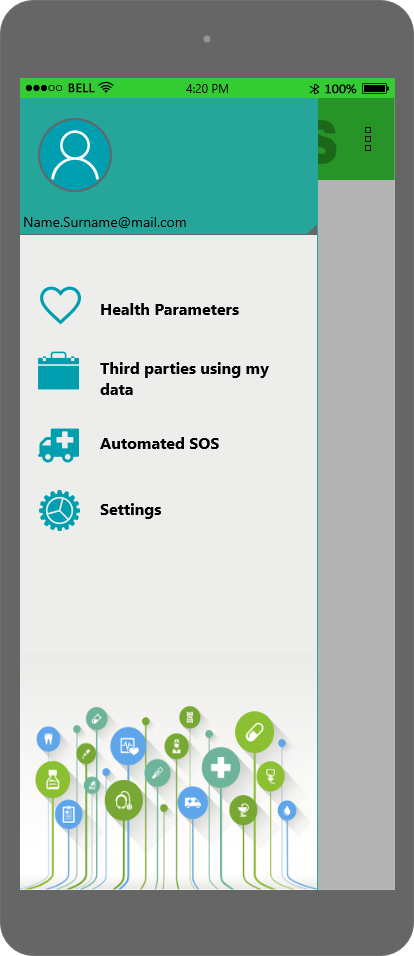
\includegraphics[width=\textwidth]{./pictures/menu.png}
    		\caption{Mock up - Menu.}
	\end{minipage}
\end{figure}

\begin{figure}[h!]
	\centering
 	\begin{minipage}[b]{0.25\textwidth}
    		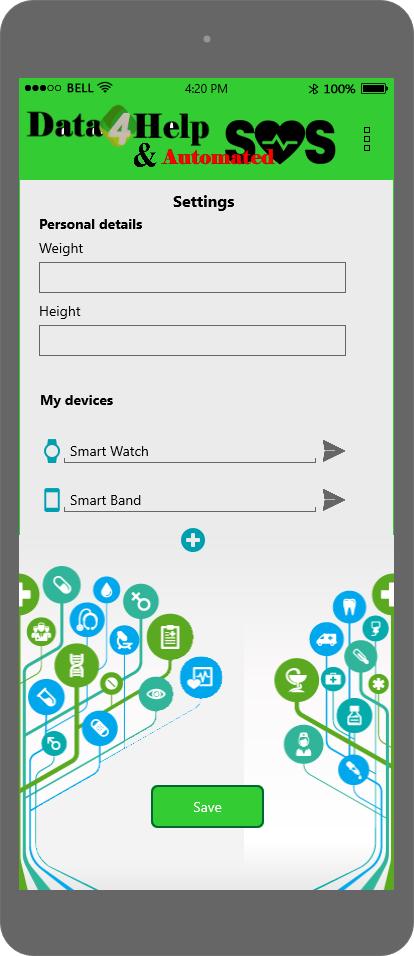
\includegraphics[width=\textwidth]{./pictures/settings.png}
    		\caption{Mock up - Settings.\\}
	\end{minipage}
	\hfill
	\begin{minipage}[b]{0.25\textwidth}
    		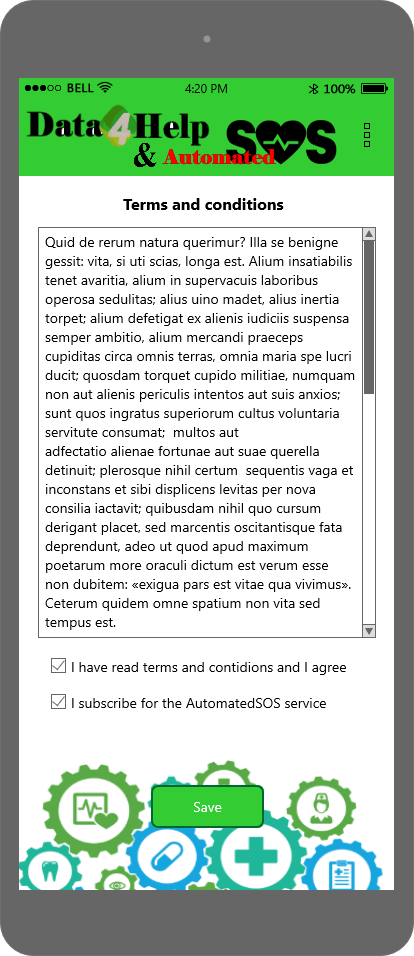
\includegraphics[width=\textwidth]{./pictures/terms_and_conditions.png}
    		\caption{Mock up - Subscribe to \textit{ASOS}.}
	\end{minipage}
	\hfill
	\begin{minipage}[b]{0.25\textwidth}
    		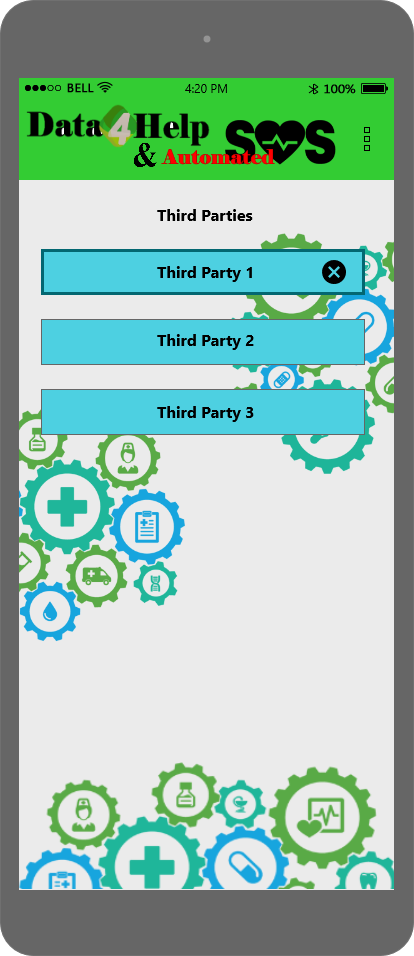
\includegraphics[width=\textwidth]{./pictures/third_party_page.png}
    		\caption{Mock up - Third party using my data.}
	\end{minipage}
\end{figure}

\begin{figure}[h!]
	\centering
 	\begin{minipage}[b]{0.25\textwidth}
    		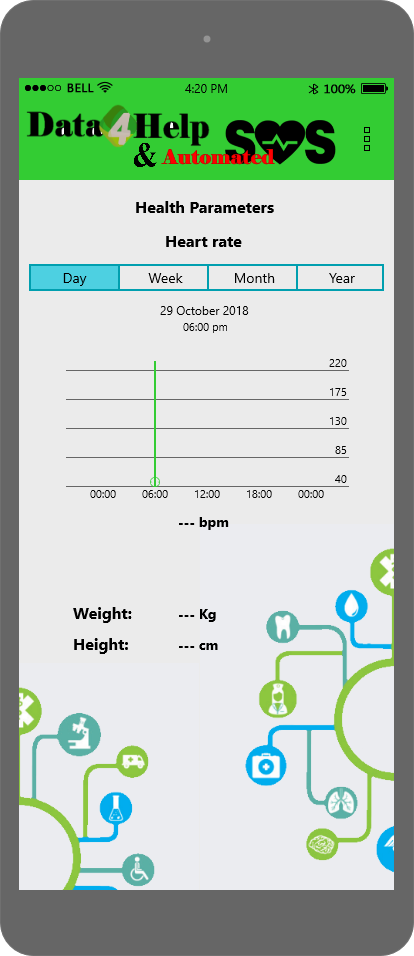
\includegraphics[width=\textwidth]{./pictures/health_param.png}
    		\caption{Mock up - Health parameter.}
	\end{minipage}
	\hfill
	\begin{minipage}[b]{0.25\textwidth}
    		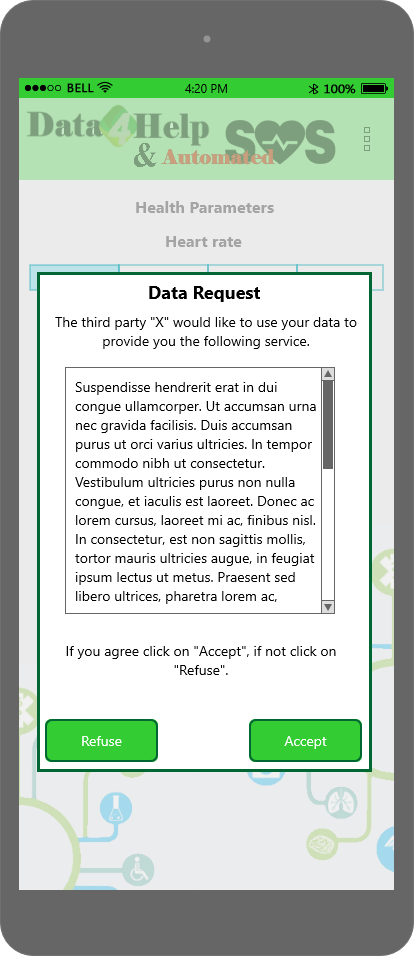
\includegraphics[width=\textwidth]{./pictures/notification.png}
    		\caption{Mock up - Allert to accept or deny .}
	\end{minipage}
\end{figure}



\subsection{Thrid Party Interface}
The following mockups represent a basic idea of how the third party's mobile app will look like in the first 
release. 

\begin{figure}[h!]
	\centering
 	 \begin{minipage}[b]{0.25\textwidth}
    		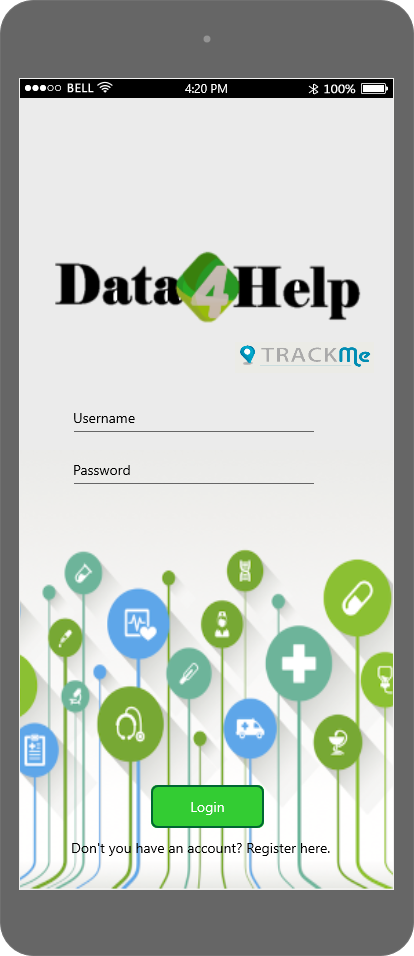
\includegraphics[width=\textwidth]{./pictures/login_3p.png}
    		\caption{Mock up - Login screen.\\}
  	\end{minipage}
	\hfill
 	\begin{minipage}[b]{0.25\textwidth}
    		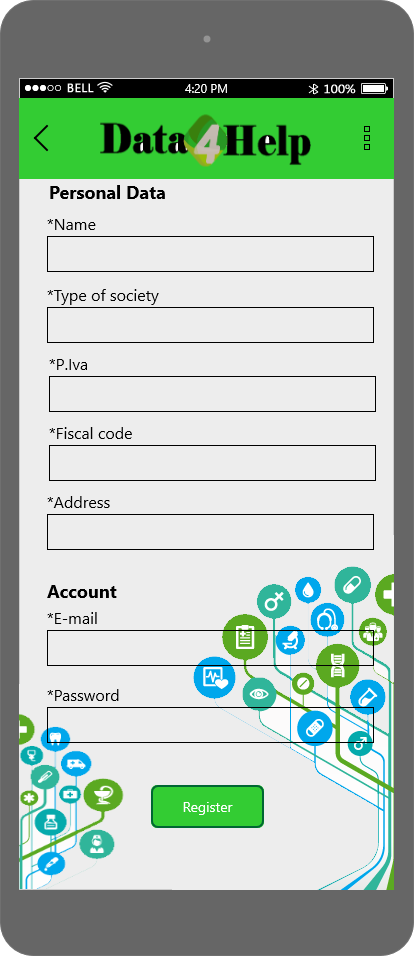
\includegraphics[width=\textwidth]{./pictures/3p_registration.png}
    		\caption{Mock up - Registration.}
	\end{minipage}
	\hfill
 	\begin{minipage}[b]{0.25\textwidth}
    		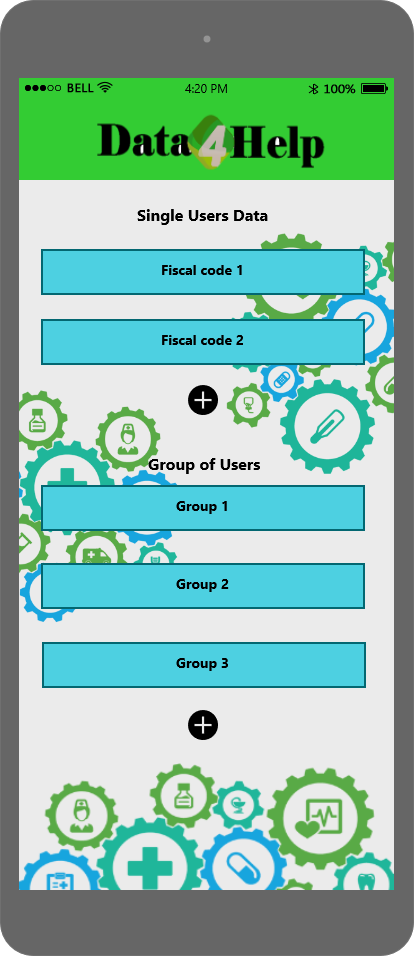
\includegraphics[width=\textwidth]{./pictures/main_scene.png}
    		\caption{Mock up - Main scene.}
	\end{minipage}
\end{figure}
 
\vspace{7cm}
   
\begin{figure}[h!]
	\centering
 	 \begin{minipage}[b]{0.25\textwidth}
    		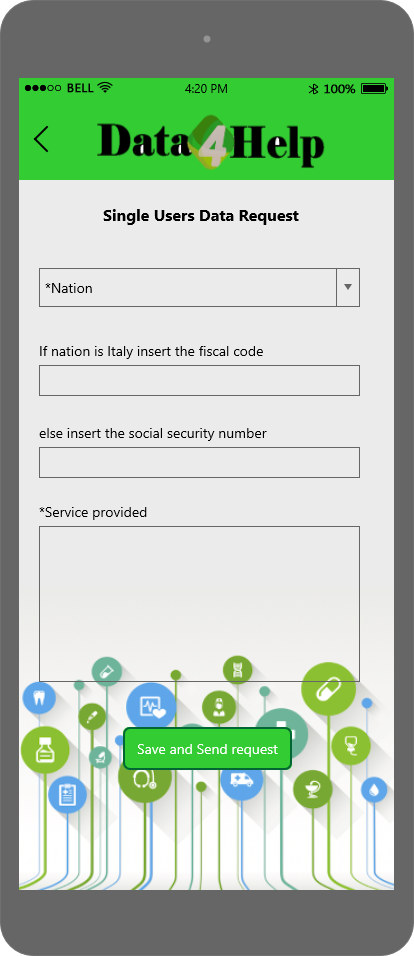
\includegraphics[width=\textwidth]{./pictures/single_user_request.png}
    		\caption{Mock up - Single data request.}
  	\end{minipage}
	\hfill
 	\begin{minipage}[b]{0.25\textwidth}
    		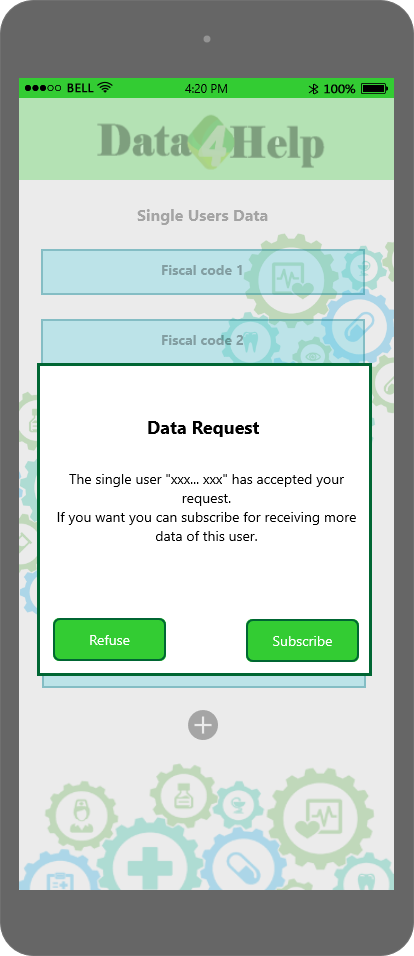
\includegraphics[width=\textwidth]{./pictures/single_user_accept.png}
    		\caption{Mock up - Positive notification.}
	\end{minipage}
	\hfill
 	\begin{minipage}[b]{0.25\textwidth}
    		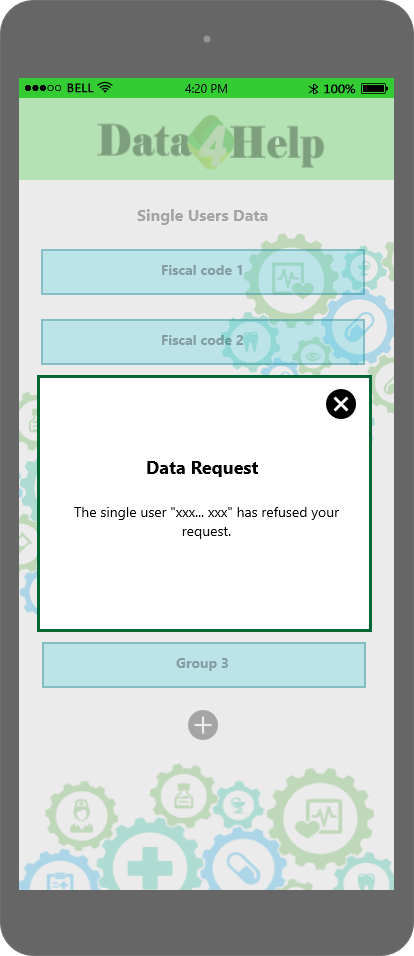
\includegraphics[width=\textwidth]{./pictures/single_user_refuse.png}
    		\caption{Mock up - Negative notification.}
	\end{minipage}
\end{figure}

\begin{figure}[h!]
	\centering
 	\begin{minipage}[b]{0.25\textwidth}
    		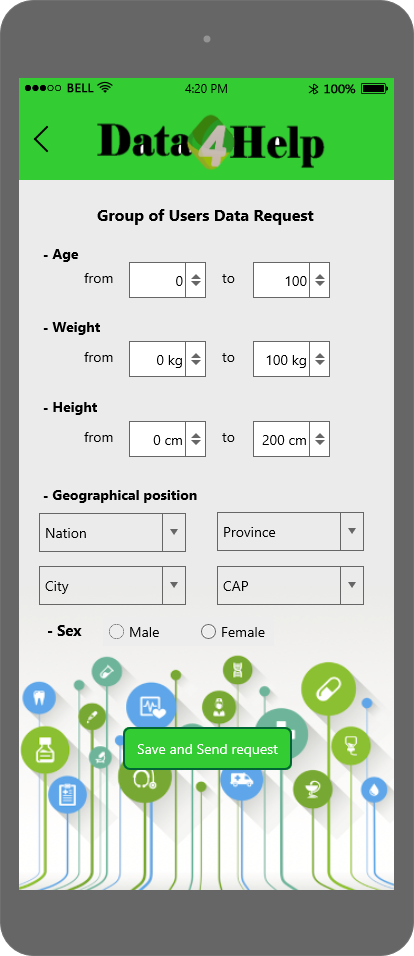
\includegraphics[width=\textwidth]{./pictures/group_request.png}
    		\caption{Mock up - Group of data request.}
	\end{minipage}
	\hfill
	\begin{minipage}[b]{0.25\textwidth}
    		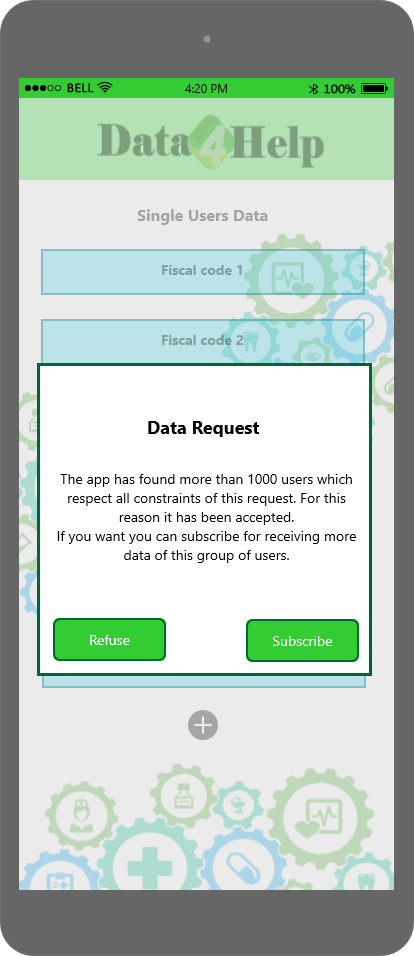
\includegraphics[width=\textwidth]{./pictures/group_accept.png}
    		\caption{Mock up - Positive notification.}
	\end{minipage}
	\hfill
	\begin{minipage}[b]{0.25\textwidth}
    		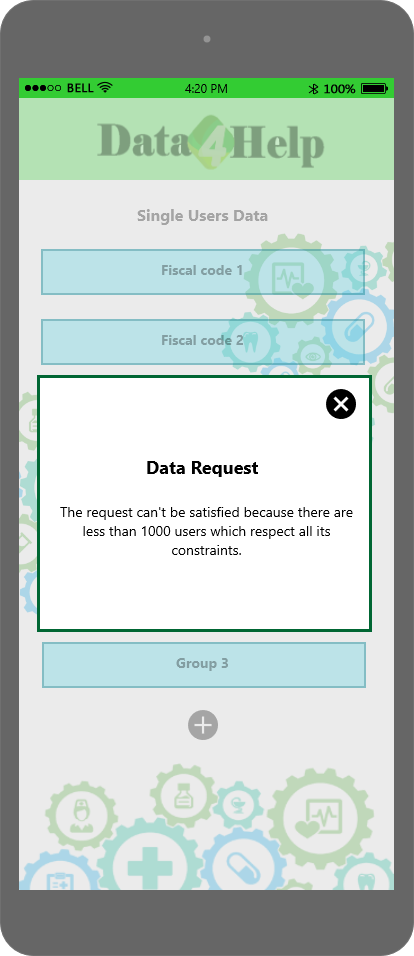
\includegraphics[width=\textwidth]{./pictures/group_refuse.png}
    		\caption{Mock up - Negative notification.}
	\end{minipage}
\end{figure}

\begin{figure}[h!]
	\centering
 	\begin{minipage}[b]{0.25\textwidth}
    		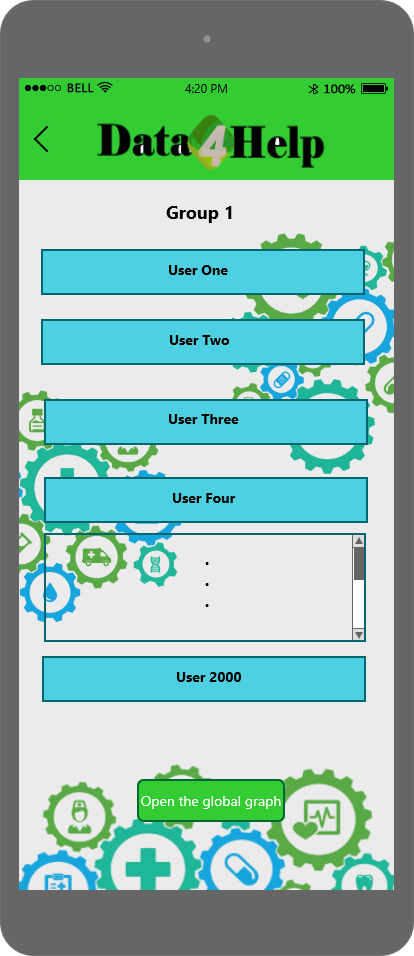
\includegraphics[width=\textwidth]{./pictures/group1.png}
    		\caption{Mock up - Users in a group.}
	\end{minipage}
	\hfill
	\begin{minipage}[b]{0.25\textwidth}
    		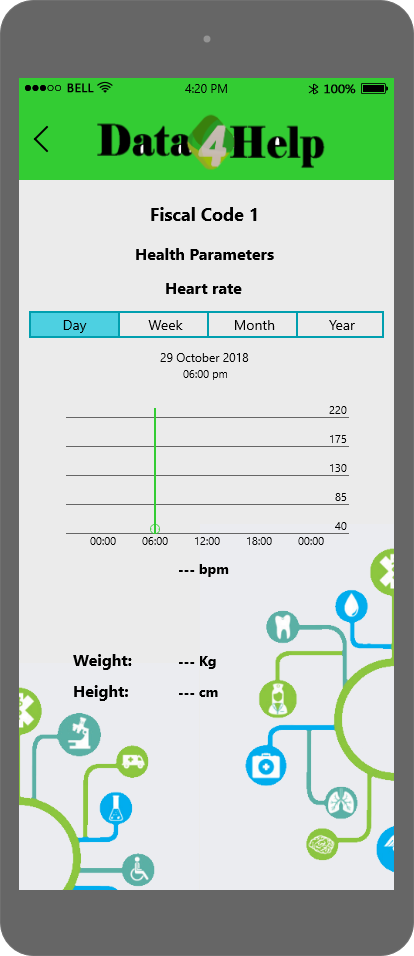
\includegraphics[width=\textwidth]{./pictures/user1.png}
    		\caption{Mock up - Single user's parameter.}
	\end{minipage}
	\hfill
	\begin{minipage}[b]{0.25\textwidth}
    		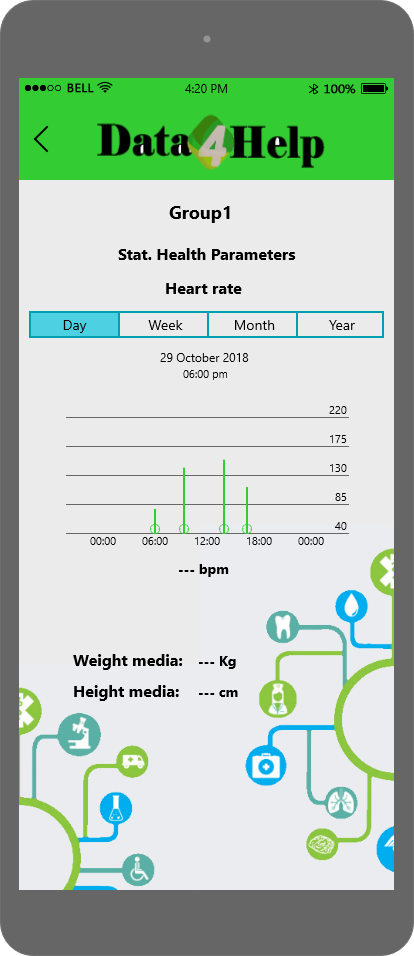
\includegraphics[width=\textwidth]{./pictures/group_stat.png}
    		\caption{Mock up - Statistic par. of a group.}
	\end{minipage}
\end{figure}

\subsection{Hardware Interface}

This is a software application whose main function is to collect data from single user, share them with third parties and give a medical service. It requires using a smartphone that can exploit GPS services to track the location and give it to the SOS service in case of unhealty users and bluetooth to connect the smartphone to the device which will collect health parameters.

\subsection{Software Interfaces}
The server side of the app needs the following software products:
\begin{itemize}
	\item Java EE (the latest available version  is the 8.2 and it is possible to download it at \url{https://goo.gl/T0IdR0});
	\item MySQL (the latest available version is the 5.7 and it can be download at \url{
	https://dev.mysql.com/downloads/mysql/5.7.html}).
\end{itemize}It is also necessary a software that will be able to automatically connect the server to the informative system of E112, the european emergency number(USA and some other states have a software which automatically redirect the E112 call to their emercency centers). By a research this software is provided only by some automobilistic houses like BMW and Volvo and by a new device called eCall that has been introduced in Europe as mandatory on vehicle of classes M1 and N1 since the 31-03-2018.

\subsection{Communication Interface}
A safe and stable communication must be always guarantee between the server and the SOS service everytime that a user becomese an unhealthy one; this is necessary in order to guarantee a really high performance and to send the correct data.
